%!TEX TS-program = xelatex

\documentclass[a4paper,12pt]{article}

%%% Работа с русским языком
\usepackage[english,russian]{babel}   %% загружает пакет многоязыковой вёрстки
\usepackage{fontspec}      %% подготавливает загрузку шрифтов Open Type, True Type и др.
\defaultfontfeatures{Ligatures={TeX},Renderer=Basic}  %% свойства шрифтов по умолчанию
\setmainfont[Ligatures={TeX,Historic}]{Calibri} %% задаёт основной шрифт документа
\setsansfont{Comic Sans MS}                    %% задаёт шрифт без засечек
\setmonofont{Courier New}
\usepackage{indentfirst}
\frenchspacing

\renewcommand{\epsilon}{\ensuremath{\varepsilon}}
\renewcommand{\phi}{\ensuremath{\varphi}}
\renewcommand{\kappa}{\ensuremath{\varkappa}}
\renewcommand{\le}{\ensuremath{\leqslant}}
\renewcommand{\leq}{\ensuremath{\leqslant}}
\renewcommand{\ge}{\ensuremath{\geqslant}}
\renewcommand{\geq}{\ensuremath{\geqslant}}
\renewcommand{\emptyset}{\varnothing}

%%% Дополнительная работа с математикой
\usepackage{amsmath,amsfonts,amssymb,amsthm,mathtools} % AMS
\usepackage{icomma} % "Умная" запятая: $0,2$ --- число, $0, 2$ --- перечисление

%% Номера формул
%\mathtoolsset{showonlyrefs=true} % Показывать номера только у тех формул, на которые есть \eqref{} в тексте.
%\usepackage{leqno} % Нумерация формул слева	

%% Перенос знаков в формулах (по Львовскому)
\newcommand*{\hm}[1]{#1\nobreak\discretionary{}
	{\hbox{$\mathsurround=0pt #1$}}{}}

%%% Работа с картинками
\usepackage{graphicx}  % Для вставки рисунков
\graphicspath{{images/}}  % папки с картинками
\setlength\fboxsep{3pt} % Отступ рамки \fbox{} от рисунка
\setlength\fboxrule{1pt} % Толщина линий рамки \fbox{}
\usepackage{wrapfig} % Обтекание рисунков текстом

%%% Работа с таблицами
\usepackage{array,tabularx,tabulary,booktabs} % Дополнительная работа с таблицами
\usepackage{longtable}  % Длинные таблицы
\usepackage{multirow} % Слияние строк в таблице
\usepackage{float}% http://ctan.org/pkg/float

%%% Программирование
\usepackage{etoolbox} % логические операторы


%%% Страница
\usepackage{extsizes} % Возможность сделать 14-й шрифт
\usepackage{geometry} % Простой способ задавать поля
\geometry{top=20mm}
\geometry{bottom=20mm}
\geometry{left=30mm}
\geometry{right=15mm}
%
%\usepackage{fancyhdr} % Колонтитулы
% 	\pagestyle{fancy}
%\renewcommand{\headrulewidth}{0pt}  % Толщина линейки, отчеркивающей верхний колонтитул
% 	\lfoot{Нижний левый}
% 	\rfoot{Нижний правый}
% 	\rhead{Верхний правый}
% 	\chead{Верхний в центре}
% 	\lhead{Верхний левый}
%	\cfoot{Нижний в центре} % По умолчанию здесь номер страницы

\usepackage{setspace} % Интерлиньяж
\onehalfspacing % Интерлиньяж 1.5
%\doublespacing % Интерлиньяж 2
%\singlespacing % Интерлиньяж 1

\usepackage{lastpage} % Узнать, сколько всего страниц в документе.

\usepackage{soul} % Модификаторы начертания

\usepackage{hyperref}
\usepackage[usenames,dvipsnames,svgnames,table,rgb]{xcolor}
\hypersetup{				% Гиперссылки
	unicode=true,           % русские буквы в раздела PDF
	pdftitle={Отчет по самостоятельной работе},   % Заголовок
	pdfauthor={Самоделкина М.В., Ремизова А.П.},      % Автор
	pdfsubject={Отчет по самостоятельной работе},      % Тема
	pdfcreator={Самоделкина М.В., Ремизова А.П.}, % Создатель
	pdfproducer={Самоделкина М.В., Ремизова А.П.}, % Производитель
	pdfkeywords={keyword1} {key2} {key3}, % Ключевые слова
	colorlinks=true,       	% false: ссылки в рамках; true: цветные ссылки
	linkcolor=blue,          % внутренние ссылки
	citecolor=black,        % на библиографию
	filecolor=magenta,      % на файлы
	urlcolor=blue           % на URL
}
\makeatletter 
\def\@biblabel#1{#1. } 
\makeatother
\usepackage{cite} % Работа с библиографией
%\usepackage[superscript]{cite} % Ссылки в верхних индексах
%\usepackage[nocompress]{cite} % 
\usepackage{csquotes} % Еще инструменты для ссылок

\usepackage{multicol} % Несколько колонок

\usepackage{tikz} % Работа с графикой
\usepackage{pgfplots}
\usepackage{pgfplotstable}

% ГОСТ заголовки
\usepackage[font=small]{caption}
%\captionsetup[table]{justification=centering, labelsep = newline} % Таблицы по правобу краю
%\captionsetup[figure]{justification=centering} % Картинки по центру
\usepackage{ dsfont }

\newcommand{\tablecaption}[1]{\addtocounter{table}{1}\small \begin{flushright}\tablename \ \thetable\end{flushright}%	
\begin{center}#1\end{center}}

\newcommand{\imref}[1]{рис.~\ref{#1}}

\usepackage{multirow}
\usepackage{spreadtab}
\newcolumntype{K}[1]{@{}>{\centering\arraybackslash}p{#1cm}@{}}


\usepackage{xparse}
\usepackage{fancyvrb}

\RecustomVerbatimCommand{\VerbatimInput}{VerbatimInput}
{
	fontsize=\footnotesize    
}

\newcolumntype{?}[1]{!{\vrule width #1}}

\usepackage{tocloft}
\renewcommand{\cftsecleader}{\cftdotfill{\cftdotsep}}

\usepackage{pdfpages}

\usepackage{longtable}

\usepackage{adjustbox}
\begin{document}
\begin{titlepage}
	\begin{center}
		ПРАВИТЕЛЬСТВО РОССИЙСКОЙ ФЕДЕРАЦИИ \\
 		ФЕДЕРАЛЬНОЕ  ГОСУДАРСТВЕННОЕ АВТОНОМНОЕ \\
		ОБРАЗОВАТЕЛЬНОЕ УЧРЕЖДЕНИЕ ВЫСШЕГО ОБРАЗОВАНИЯ\\
		«НАЦИОНАЛЬНЫЙ ИССЛЕДОВАТЕЛЬСКИЙ УНИВЕРСИТЕТ\\
		«ВЫСШАЯ ШКОЛА ЭКОНОМИКИ»
	\end{center}
	
	\begin{center}
		\textbf{Московский институт электроники и математики}
		
		\textbf{Им. А.Н.Тихонова НИУ ВШЭ}
		
		\vspace{2ex}
		
		\textbf{Направление 01.03.04. Прикладная математика \\
			Бакалаврская программа <<Прикладная математика>>}
	\end{center}
	\vspace{1ex}	
	
	\vspace{1ex}
	\begin{center}
		\textbf{Отчет по самостоятельной работе \\
			по дисциплине <<Методы анализа стохастических взаимосвязей>>\\
			часть 2
	}
	\end{center}	

	\vspace{2ex}
	\vfill
	
	\vspace{2ex}
	
	\begin{flushright}
		\textbf{Бригада №7:}
		
		\vspace{2ex}
		
		Ремизова Анна Петровна, 4 курс, БПМ174
		
		Самоделкина Мария Владимировна, 4 курс, БПМ174

	\end{flushright}

	\vspace{5ex}
	\begin{center}
		Москва \the\year \, г.
	\end{center}
	
\end{titlepage}
\addtocounter{page}{1}
\tableofcontents
\pagebreak

\section{Описание данных}
% Период времени и тип данных
Частота измерений каждые 4 секунды. Величину стандартного интервала наблюдений принимаем равным среднему времени прохождения спортсменом одного круга (около 6 минут).

% Гипотезы

\subsection{Зависимая переменная Пульс}
% Определение
\begin{figure}[H]
	\centering
	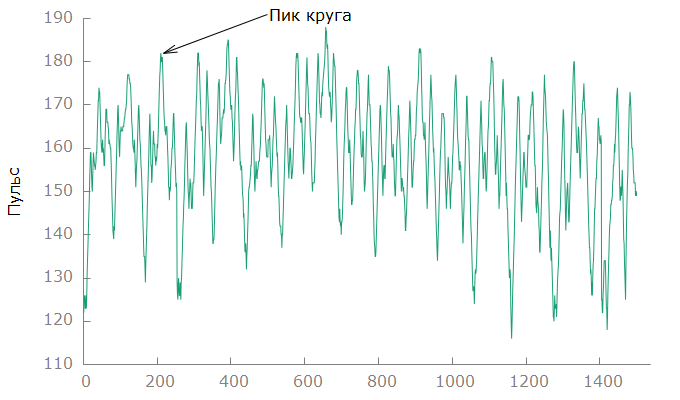
\includegraphics[width=0.7\linewidth]{../[graphics]/hr_graph}
	\caption{График зависимой переменной Пульс}
	\label{fig:hr_graph}
\end{figure}

% Анализ автокорреляции
\textbf{\textit{Анализ автокорреляции}}

\begin{figure}[H]
	\centering
	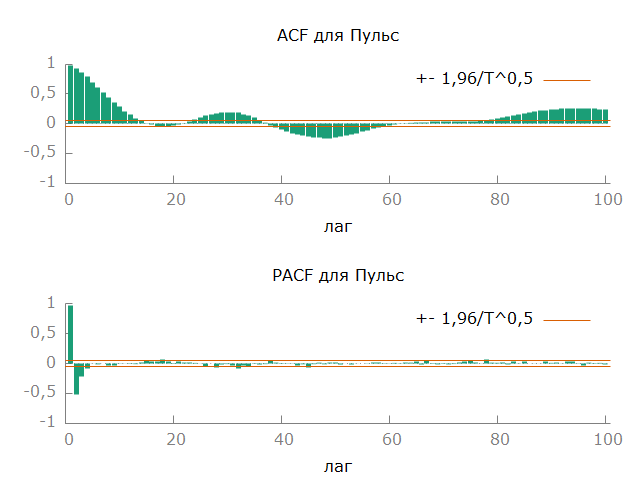
\includegraphics[width=0.7\linewidth]{../[graphics]/hr_acf_100}
	\caption{Графики ACF и PACF зависимой переменной Пульс}
	\label{fig:hr_acf_100}
\end{figure}

График автокорреляции (рис. \ref{fig:hr_acf_100}) убывает медленно, предполагается наличие тренда. На графике видны колебания с периодом в треть круга (лаг 30), полкруга (лаг 45) и круг (лаг 88). При анализе графика значений зависимой переменной (рис. \ref{fig:hr_graph}) также хорошо видны круговые колебания. По виду графиков можно говорить о наличии периодического тренда с периодом, равным среднему времени прохождения спортсменом круга.

% Анализ спектрограммы
\textbf{\textit{Анализ спектрограммы}}

\begin{figure}[H]
	\centering
	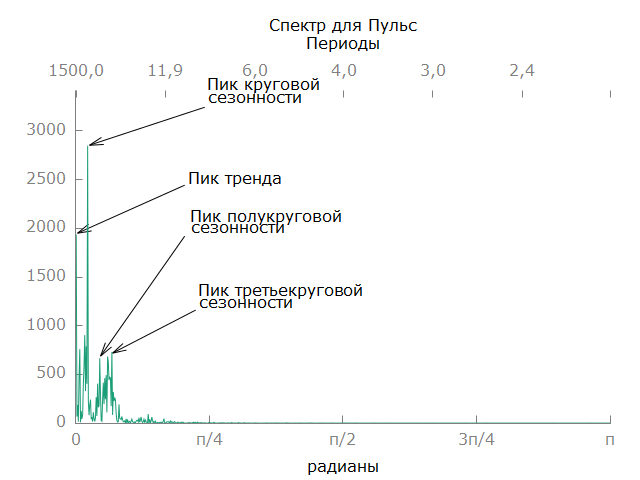
\includegraphics[width=0.7\linewidth]{../[graphics]/hr_spectr}
	\caption{График периодограммы зависимой переменной Пульс}
	\label{fig:hr_spectr}
\end{figure}

При анализе графика (рис. \ref{fig:hr_spectr}) видны пики вблизи нулевой частоты, они свидетельствуют о потенциальном наличии долгосрочного тренда. На графике также видны несколько пиков в циклической области спектра, следовательно, в данном ряде могут присутствовать циклы. 
В сезонной части спектра на частоте $f = 0,07121 \approx \frac{\pi}{44}$ значение спектральной частоты равно $Sd = 2847,9$, указанная частота соответствует периоду круга. 
На частоте $f = 0,14242 \approx \frac{\pi}{22}$ значение спектральной частоты равно $Sd = 665,40$, указанная частота соответствует периоду полукруга. 
На частоте $f = 0,21363 \approx \frac{\pi}{15}$ значение спектральной частоты равно $Sd = 730,46$, указанная частота соответствует периоду в треть круга. Гармоническая составляющая в указанном ряду является хорошо выраженной.

% Анализ стационарности с использованием критерия Dickey-Fuller

%Выводы
\textbf{\textit{Выводы}}

Наличие долгосрочного тренда зависимой переменной Пульса объясняется тем, что с течением времени тренировки спортсмен устает, вследствие чего пульс постепенно увеличивается. Наличие кругового тренда объясняется тем, что рельеф местности каждый круг повторяется. Наличие сезонной частоты с периодом, равным половине круга связано с особенностями местности: каждые полкруга высота траектории движения сначала возрастала, а затем убывала. Наличие сезонной частоты с периодом, равным трети круга связано с периодичной сменой техники передвижения. %TODO

\subsection{Независимые переменные}
\subsubsection{Высота}
% Определение
\begin{figure}[H]
	\centering
	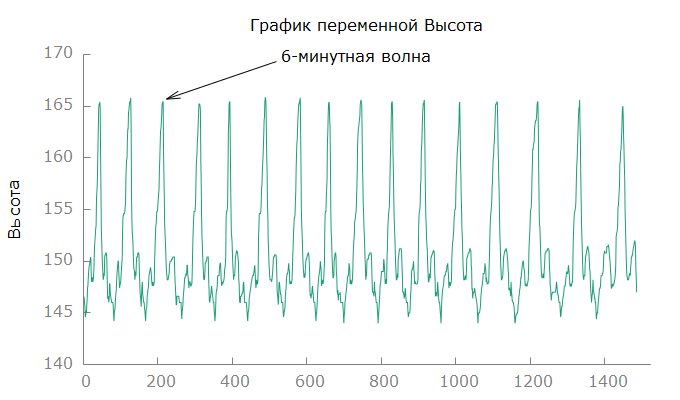
\includegraphics[width=0.7\linewidth]{../[graphics]/ele_graph}
	\caption{График зависимой Высота}
	\label{fig:ele_graph}
\end{figure}

% Анализ автокорреляции
\textbf{\textit{Анализ автокорреляции}}

\begin{figure}[H]
	\centering
	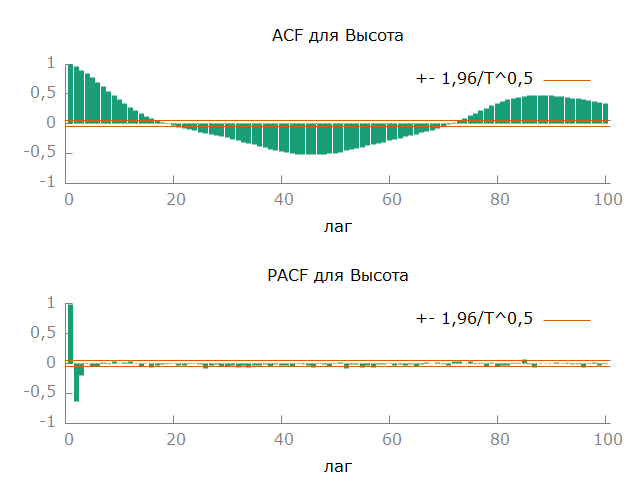
\includegraphics[width=0.7\linewidth]{../[graphics]/ele_acf_100}
	\caption{Графики ACF и PACF переменной Высота}
	\label{fig:ele_acf_100}
\end{figure}

График автокорреляции (рис. \ref{fig:ele_acf_100}) убывает медленно, предполагается наличие тренда. На графике видны колебания с периодом полкруга (лаг 45) и круг (лаг 88). При анализе графика значений переменной (рис. \ref{fig:ele_graph}) также хорошо видны круговые колебания. По виду графиков можно говорить о наличии периодического тренда с периодом, равным среднему времени прохождения спортсменом круга.

% Анализ спектрограммы
\textbf{\textit{Анализ спектрограммы}}

\begin{figure}[H]
	\centering
	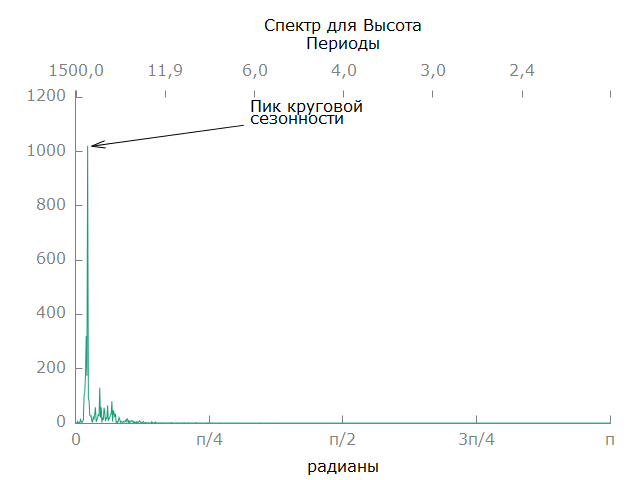
\includegraphics[width=0.7\linewidth]{../[graphics]/ele_spectr}
	\caption{График периодограммы переменной Высота}
	\label{fig:ele_spectr}
\end{figure}

При анализе графика (рис. \ref{fig:hr_spectr}) видно, что пики вблизи нулевой частоты отсутствуют, долгосрочного тренда нет. На графике отсутствуют пики в циклической области спектра. 
В сезонной части спектра на частоте $f = 0,07121 \approx \frac{\pi}{44}$ значение спектральной частоты равно $Sd = 1021,2$, указанная частота соответствует периоду круга. У данного ряда есть ярковыраженная сезонная составляющая.
Также имеются другие неярковыраженные пики в сезонной части спектра.

% Анализ стационарности с использованием критерия Dickey-Fuller

%Выводы
\textbf{\textit{Выводы}}

Долгосрочного тренда в рассматриваемом ряде быть не должно: спортсмен каждый круг проезжал по одной и той же территории, высота не изменялась. 
Однако тренд в течение круга есть. Видно, что за круг высота сначала растет, а потом практически симметрично падает. Такая симметрия связана с особенностями местности, на которой снимались показания.
Наличие кругового тренда объясняется тем, что рельеф местности каждый круг повторяется. Однако в изменениях высоты могут присутствовать незначительные колебания из-за того, что спортсмен каждый раз мог выбирать незначительно отличающуюся траекторию.

\subsubsection{Каденс}
% Определение
\begin{figure}[H]
	\centering
	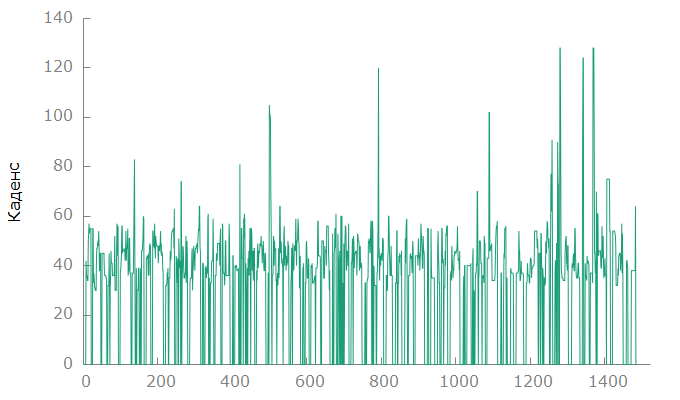
\includegraphics[width=0.7\linewidth]{../[graphics]/cad_graph}
	\caption{График зависимой Каденс}
	\label{fig:cad_graph}
\end{figure}

% Анализ автокорреляции
\textbf{\textit{Анализ автокорреляции}}

\begin{figure}[H]
	\centering
	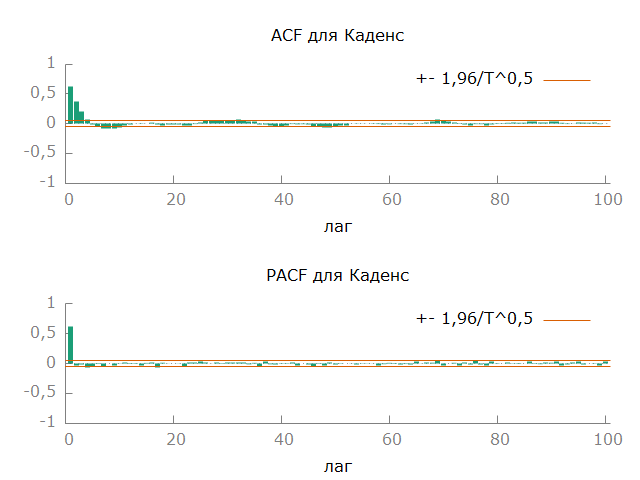
\includegraphics[width=0.7\linewidth]{../[graphics]/cad_acf_100}
	\caption{Графики ACF и PACF переменной Каденс}
	\label{fig:cad_acf_100}
\end{figure}

График автокорреляции (рис. \ref{fig:cad_acf_100}) убывает быстро, предполагается отсутствие тренда. Влияние сезонности предположительно отсутствует.

% Анализ спектрограммы
\textbf{\textit{Анализ спектрограммы}}

\begin{figure}[H]
	\centering
	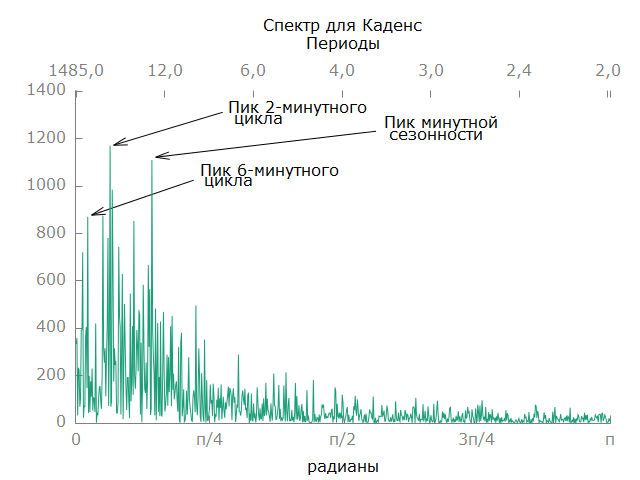
\includegraphics[width=0.7\linewidth]{../[graphics]/cad_spectr}
	\caption{График периодограммы переменной Каденс}
	\label{fig:cad_spectr}
\end{figure}

При анализе графика (рис. \ref{fig:cad_spectr}) видно, что пики вблизи нулевой частоты отсутствуют, долгосрочного тренда нет. На графике присутствуют пики в циклической области спектра. 
В сезонной части спектра на частоте $f = 0,21782 \approx \frac{\pi}{14}$ значение спектральной частоты равно $Sd = 1331,6$, указанная частота соответствует периоду трети круга.
Также имеются другие пики в сезонной части спектра.

% Анализ стационарности с использованием критерия Dickey-Fuller

%Выводы
\textbf{\textit{Выводы}}

Отсутствие тренда связано с тем, что используемая в конкретный момент техника передвижения спортсмена практически не зависит от техники, используемой в предыдущие моменты времени.
Наличие сезонной частоты с периодом, равным трети круга связано с периодичностью применяемой техники передвижения. %TODO

\subsubsection{Сезонные переменные}

\end{document} % конец документа